% $Id$

\subsection{\label{ssec:high-arch}High-level \emph{vic} Architecture}

We have drawn a high-level overview of \emph{vic} architecture (sender only)
that has congestion control modules as in Figure~\ref{fig:high-vic-arch}. This
figure represents a high-level overview of \emph{vic} so that we could see the
major components of the system, and how they are interacting with each other. 

\vspace{1cm}

\begin{figure}[!h]
\begin{center}
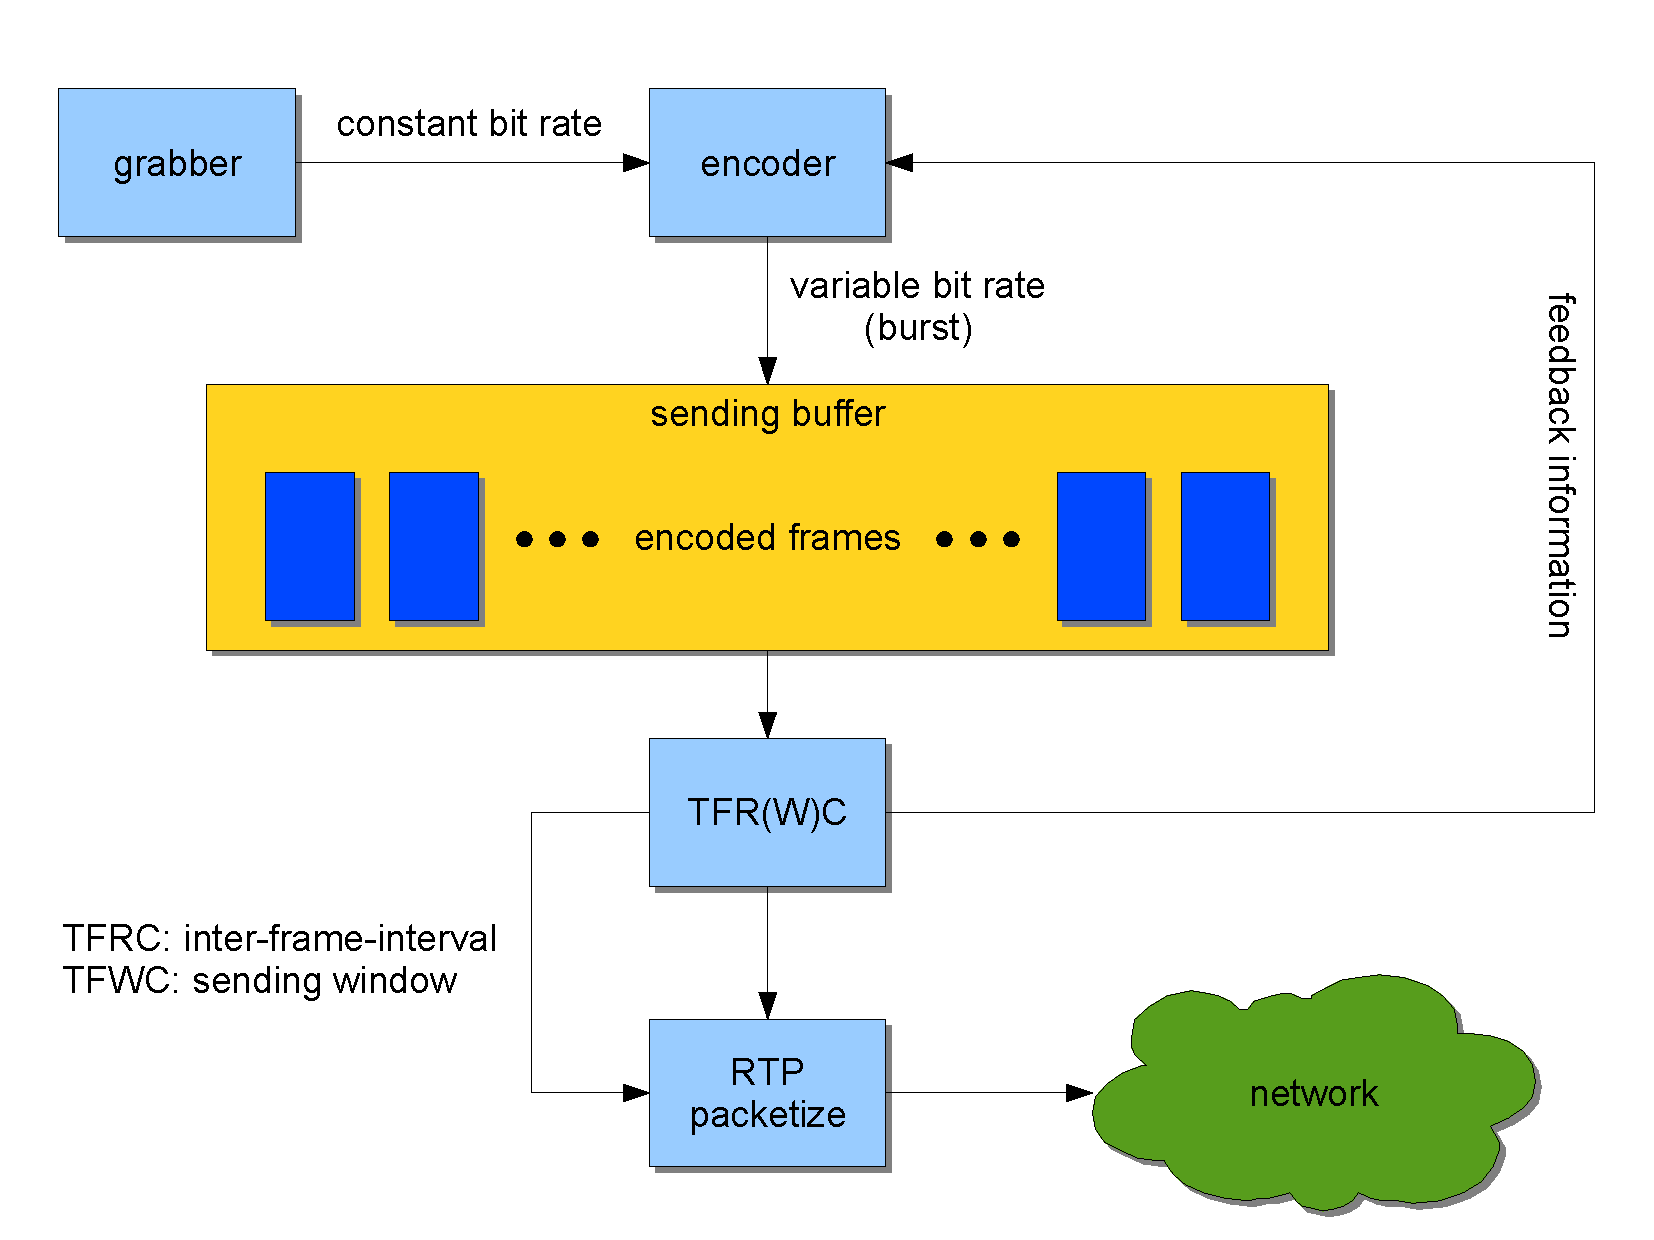
\includegraphics[scale=.5]{./img/high-vic-arch}
\caption{\label{fig:high-vic-arch}High-level Overview \emph{vic} Architecture 
with CC Mechanisms}
\end{center}
\end{figure}

Unlike to the sender, we envisage the architecture of the receiver is relatively
simple. For example, upon a packet reception, it will be inserted to a receive
buffer, subsequently decoded (and some color conversion if necessary), and
finally displayed in a output device. Depending upon a codec, the rendered
frames may not be discareded immediately, but will be kept for some times before
they get purged.

\subsection{\label{ssec:vic-overview}\emph{vic} Overview by Example}

In this subsection, we describe how \emph{vic} works. To do so, we take the
still grabber (\texttt{grabber-still.cpp}) as an example and describe how
packets are transmitted.  The purpose of this analysis is to figure out how
\emph{vic} works and, from that, we would like to know how to design the
congestion control APIs.  Figure~\ref{fig:still-grabber} shows a class-diagram
like figure that how the still grabber generates packets.

\begin{figure}[!h] 
\begin{center}
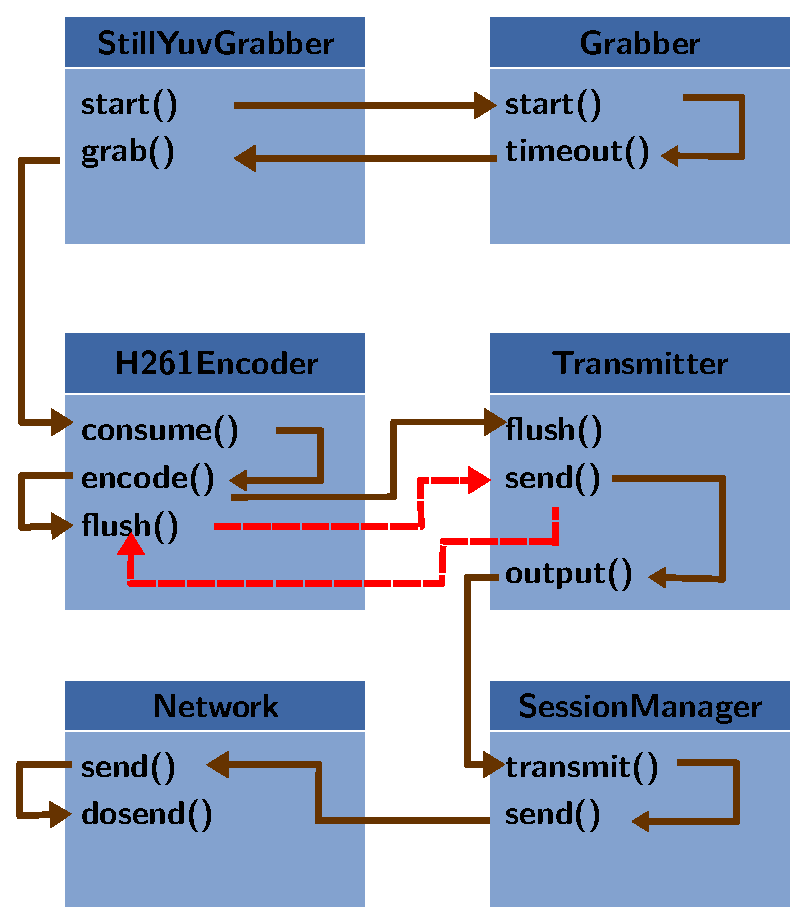
\includegraphics[scale=.5]{./img/still-grabber}
\caption{\label{fig:still-grabber}Still Grabber Information Flow}
\end{center} 
\end{figure}

The still grabber can be used when we want to feed pre-recored video sequences
to the \emph{vic} system\footnote{One should start \emph{vic} using the
following command: \texttt{./vic -XstillGrabber \emph{(IP address)}/\emph{(port
number)}}.}. Currently, the still grabber in \emph{vic} can take a JPG image
file (4:2:2) and a CIF formatted video file.

Once the still device loads a file (either a JPG or a CIF file) into the memory,
it invokes \texttt{StillGrabber} or \texttt{StillYuvGrabber} depending upon a
file type. Assuming \texttt{StillYuvGrabber} is called, it sets the frame size
by calling \texttt{setsize()} method, and call \texttt{StillYuvGrabber::start()}
wich again calls \texttt{Grabber::start()}.  \texttt{Grabber::start()} basically
sets a frame clock and sets \texttt{timeout()}. Then,
\texttt{StillYuvGrabber::grab()} starts grabbing video frames from the memory
and passes to the encoder (\texttt{encoder-h261.cpp}): in this case,
\texttt{H261PixelEncoder::consume()} will be called. After that, it starts
encoding macro-blocks given a set of YUV inputs and send the packets.

\newpage
